



\section{Experimentación}
    \subsection{Pruebas con filtro de Mahony y MPU-9250}
       A continuación se muestran algunas de las pruebas que se hiceron usando en conjunto el 
       MPU-9250 y el filtro de Mahony. Donde con el MPU-9250 obtendremos mediciones de sus 3 sensores internos, acelerómetro, 
       giroscopio y magnetómetro, las fusionaremos y usaremos el filtro de Mahony que 
       implementamos para así poder obtener la orientación actual del bebé.

       \begin{figure}[htp!]
        \centering
             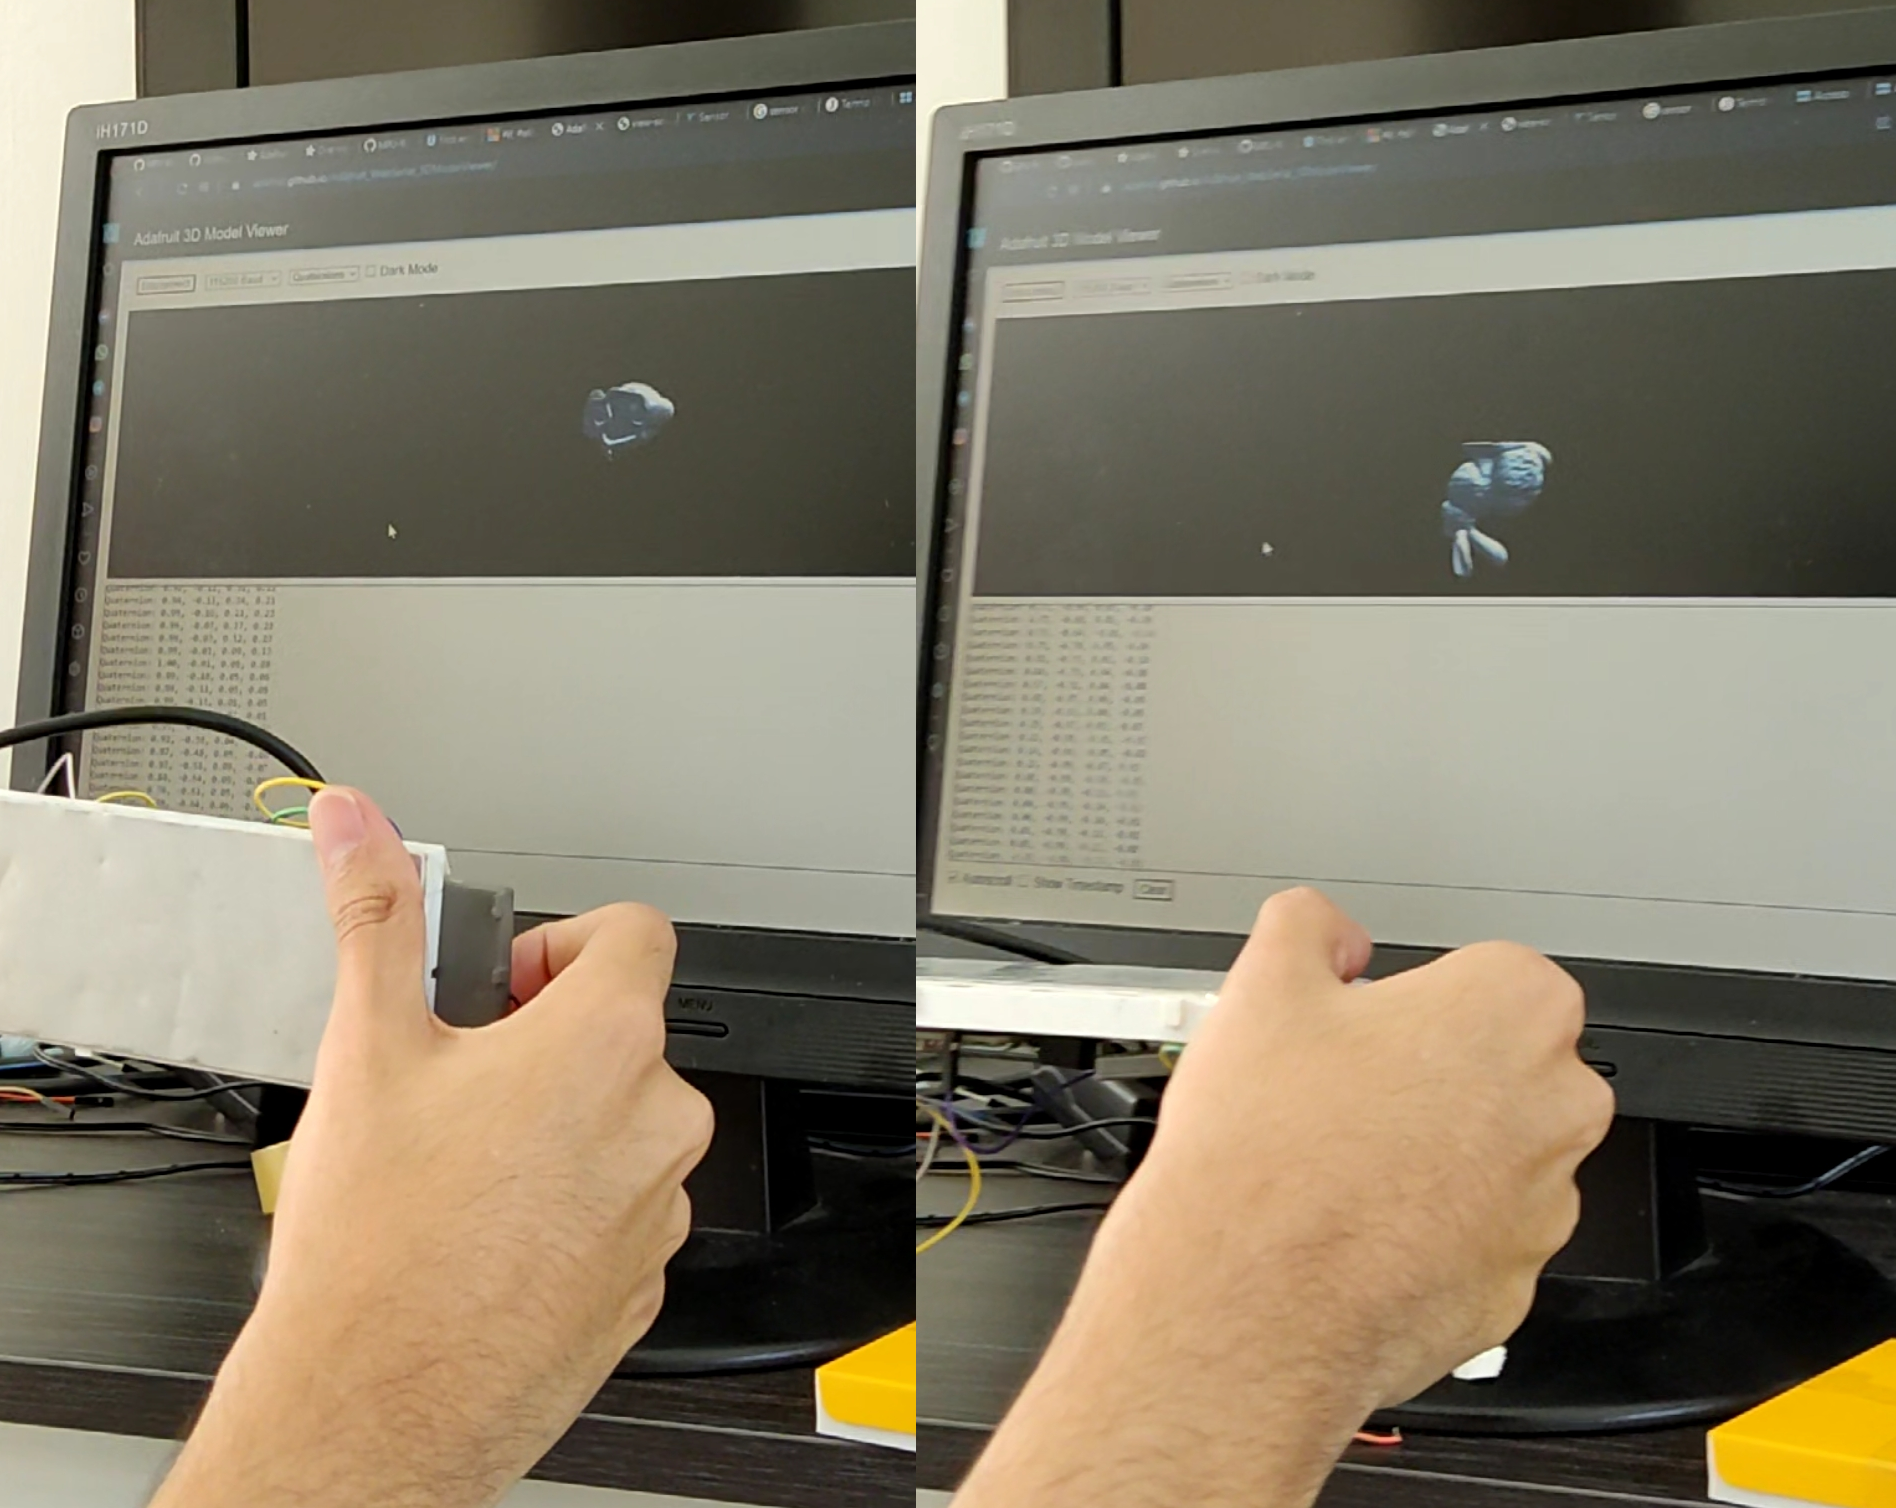
\includegraphics[width=\columnwidth]{mahony_filter_mpu_9250_y_axis_test.png}
              \caption{Prueba de orientación en el eje-Y utilizando el MPU-9250 y el filtro Mahony}
              \label{fig: test-y}
        \end{figure}
        \FloatBarrier 

        En la figura \ref{fig: test-y} se muestra el circuito en un ángulo de 90 y 180 grados en el eje Y, simulando que el bebé
        esta acostado de lado y boca abajo respectivamente, las cuales son posiciones peligrosas para el bebé, especialmente
        la segunda.

        \begin{figure}[htp!]
        \centering
            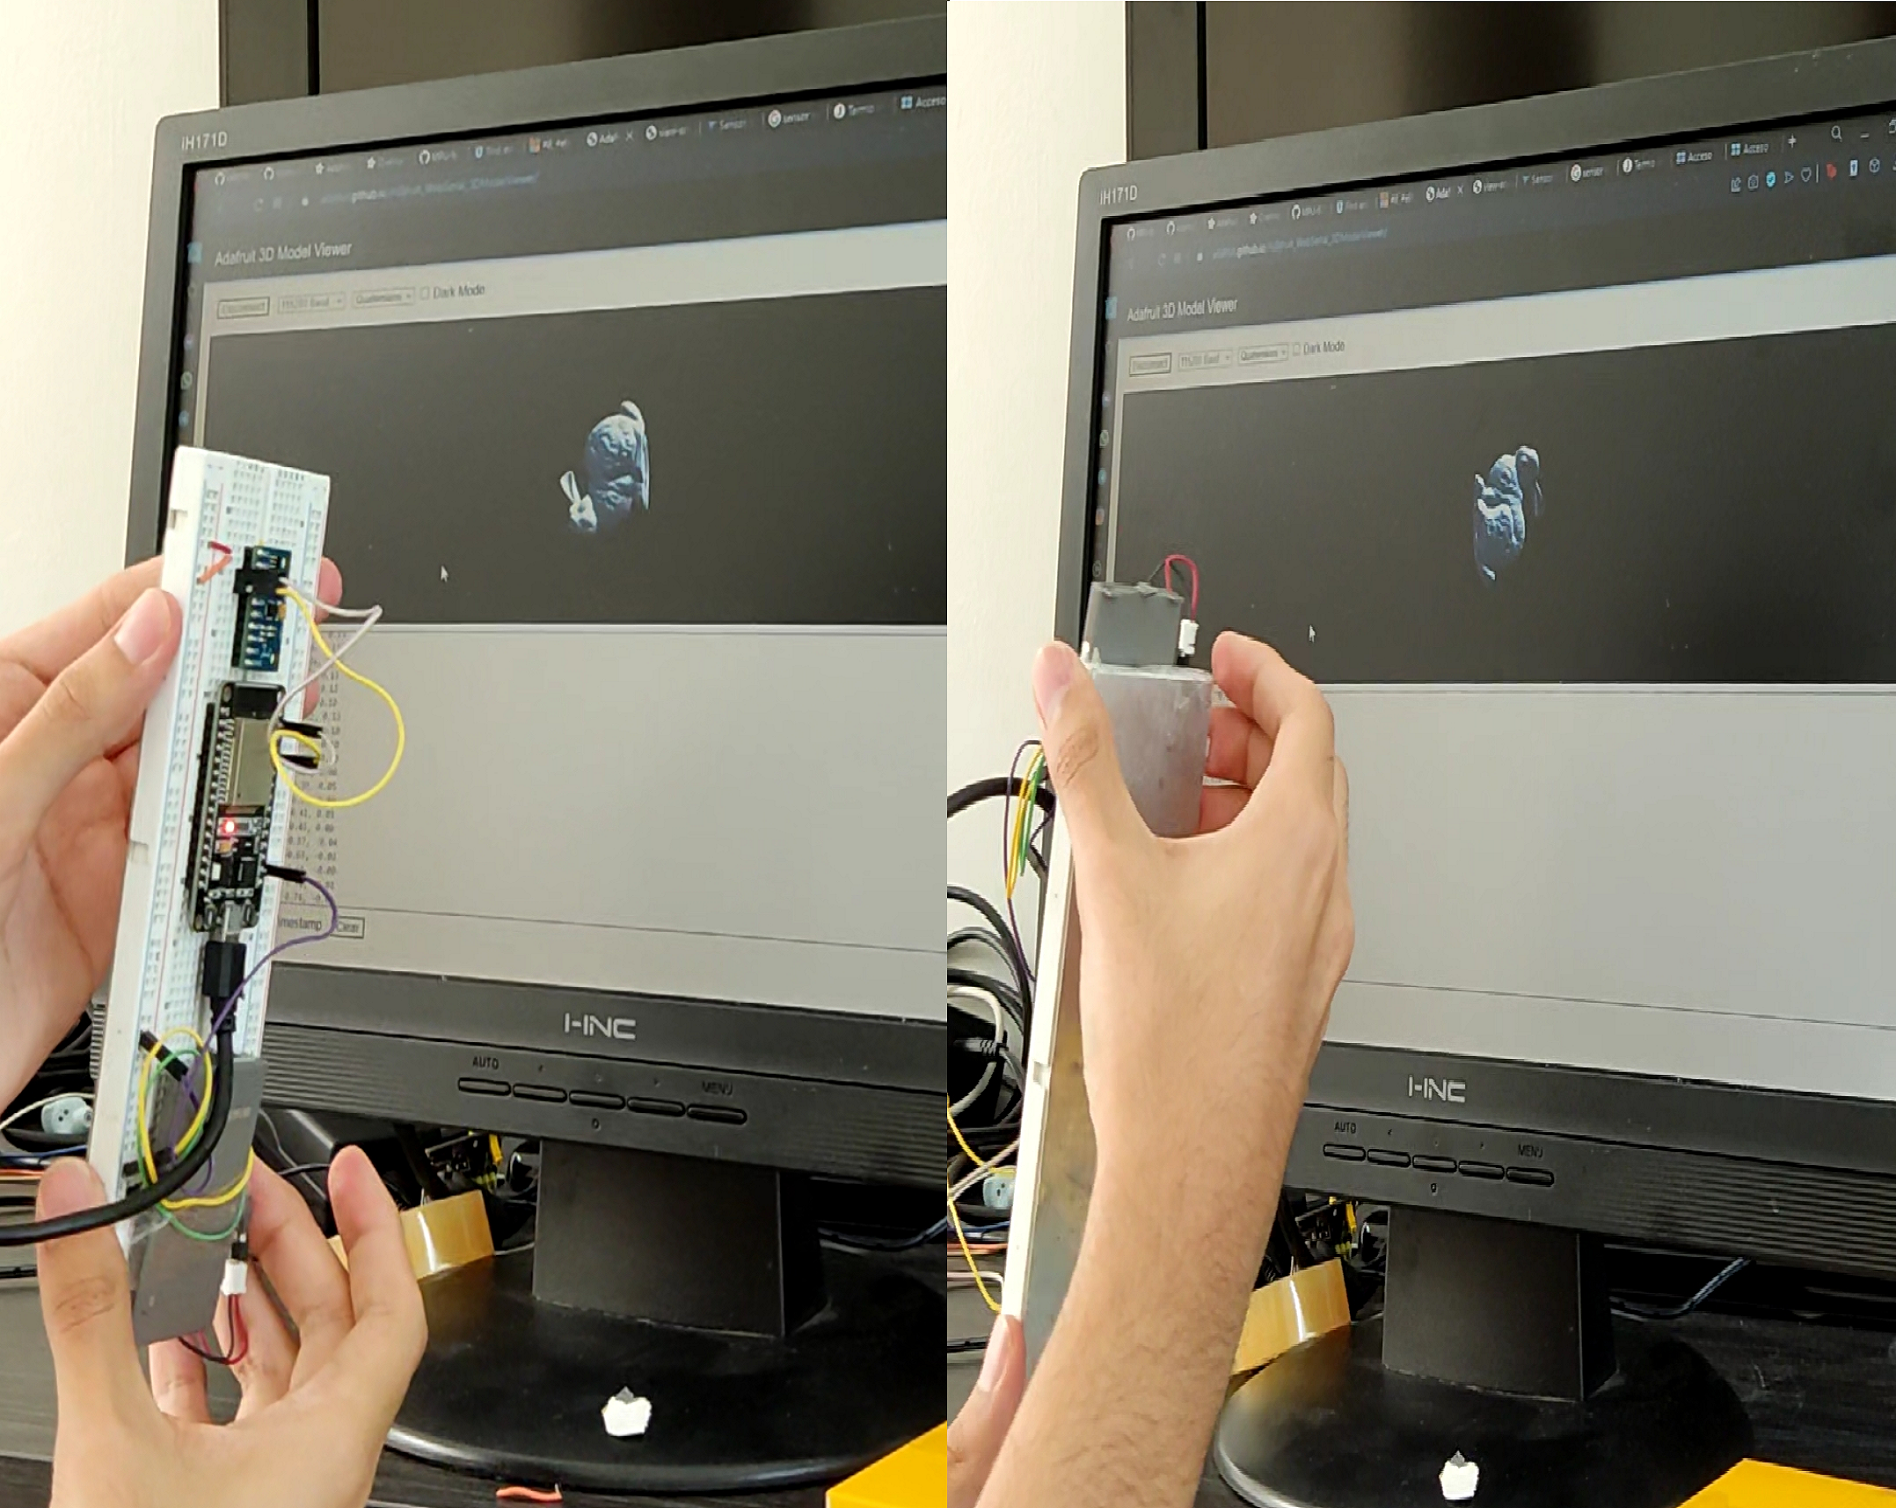
\includegraphics[width=\columnwidth]{mahony_filter_mpu_9250_x_axis_test.png}
            \caption{Prueba de orientación en el eje-X utilizando el MPU-9250 y el filtro Mahony}
            \label{fig: test-x}
        \end{figure}
        \FloatBarrier 
    
        En la figura \ref{fig: test-x} se muestra el circuito en un ángulo de 90 y -90 grados en el eje X, simulando que el bebé
        esta sentado.

        \begin{figure}[htp!]
        \centering
            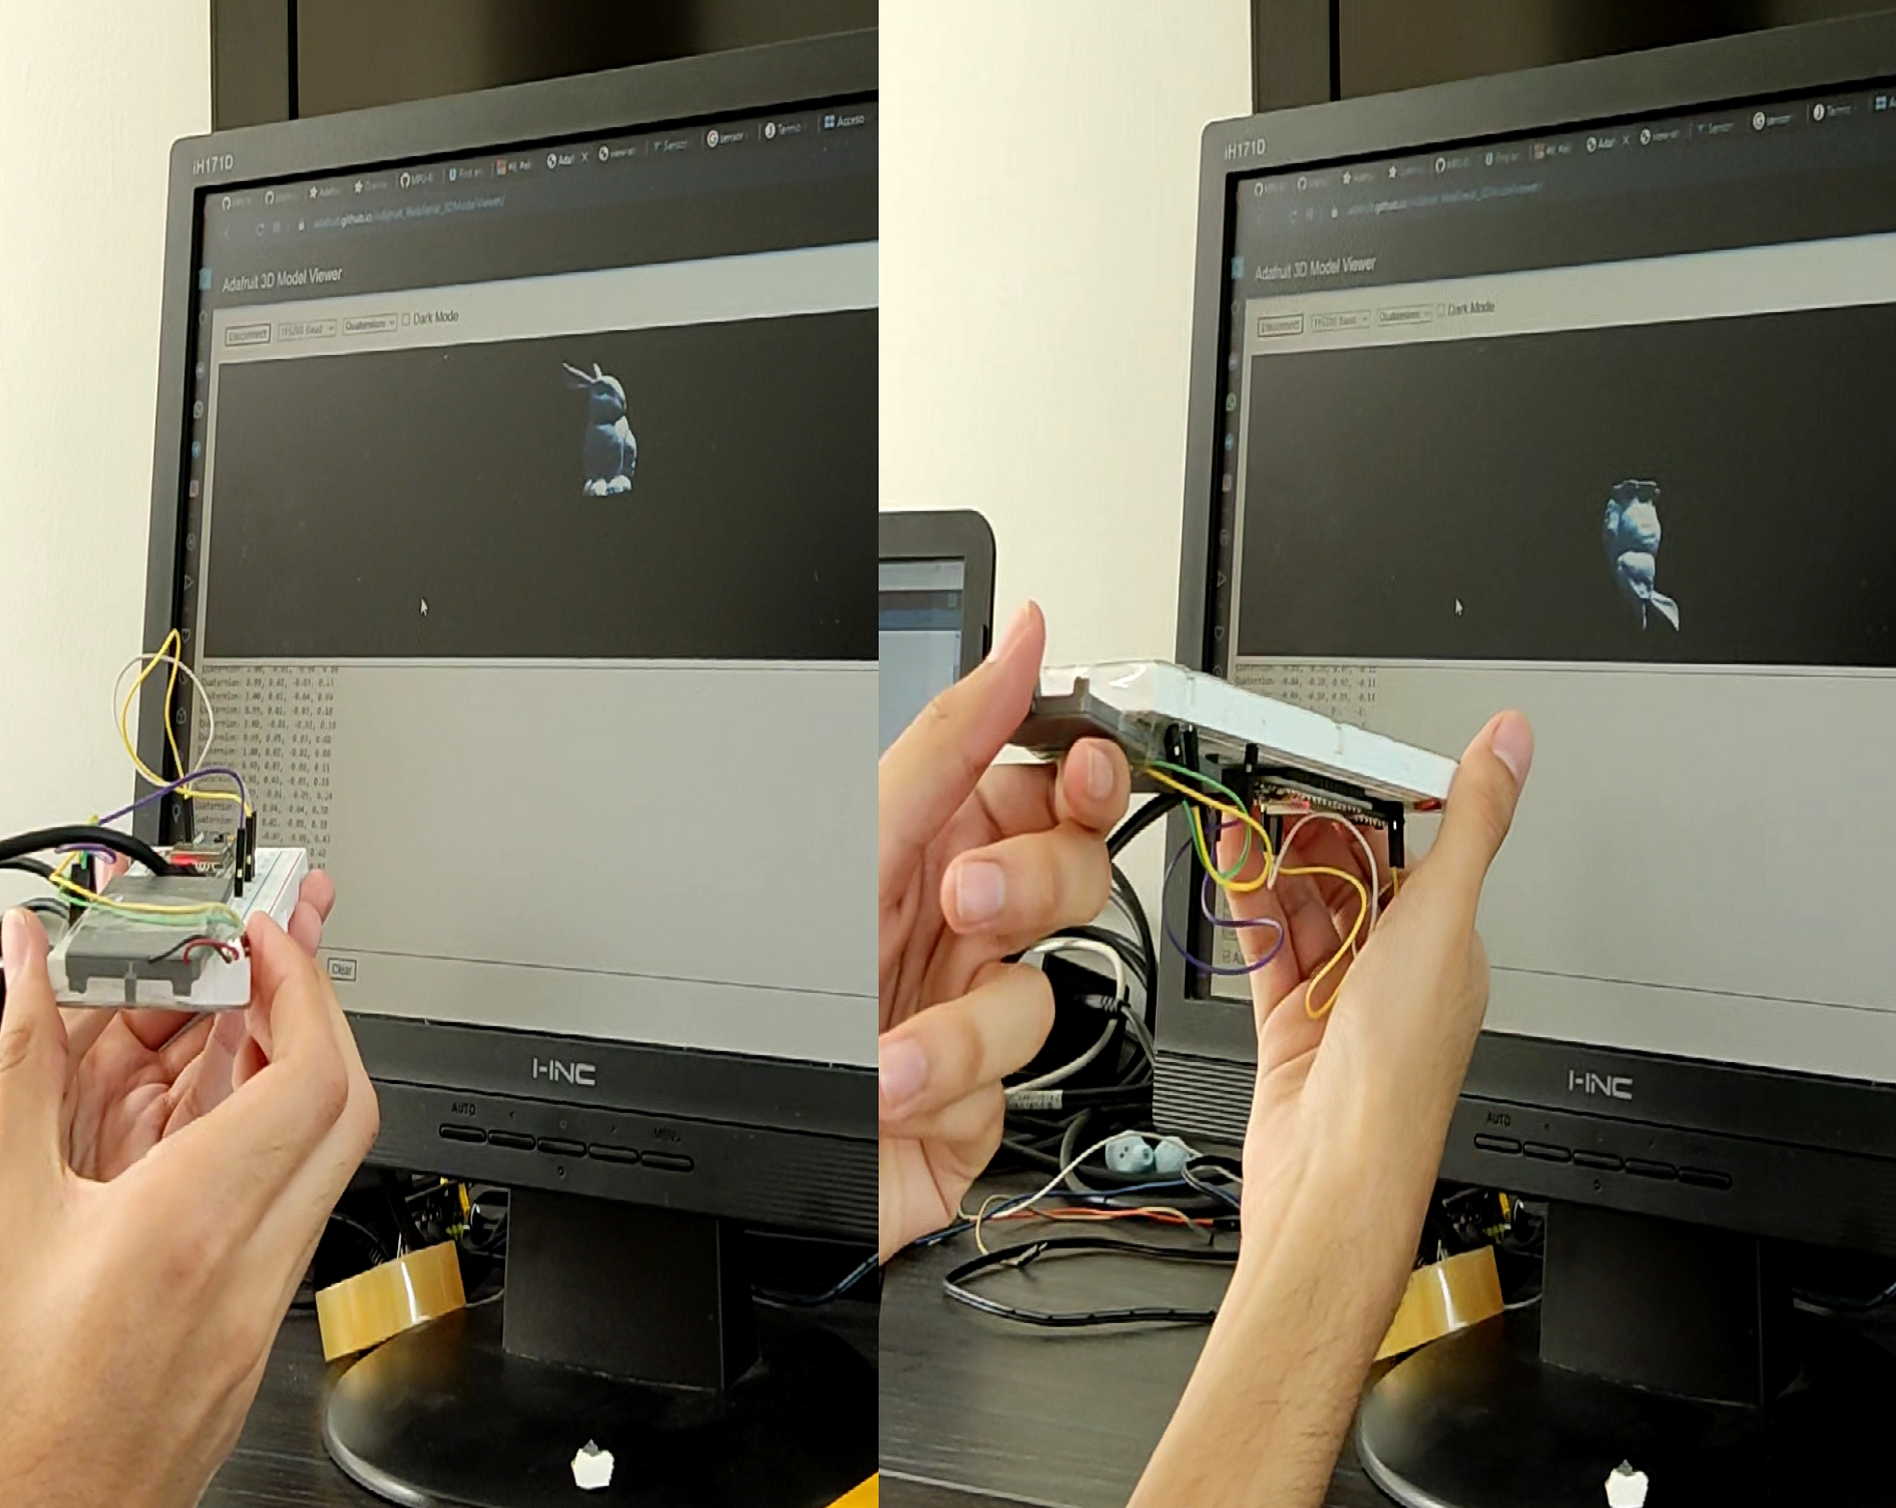
\includegraphics[width=\columnwidth]{mahony_filter_mpu_9250_z_axis_test.png}
            \caption{Prueba de orientación en el eje-Z utilizando el MPU-9250 y el filtro Mahony}
            \label{fig: test-z}
        \end{figure}
        \FloatBarrier 

        En la figura \ref{fig: test-z} se muestra el circuito viendo hacia arriba y hacia abajo, con diferentes rotaciones en el eje y,
        simulando que el bebé ha girado sobre su propio eje estando boca arriba (posición supina) y boca abajo (posición prona), donde estas
        dos situaciones son peligrosas, especialmente la segunda.\newline

        \textbf{Diagrama de conexión para el circuito}
        \begin{figure}[htp!]
            \centering
                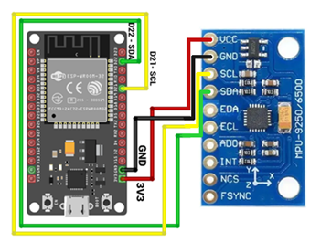
\includegraphics[width = 0.35 \textwidth]{wiring_diagram_mpu_9250_mahony_filter.png}
                \caption{Diagrama de conexiones entre el ESP32 y el MPU-9250}
            \end{figure}
            \FloatBarrier 
        \textbf{Código prueba}

        \lstset{style=mystyle}

        \lstinputlisting[language=C++, numbers=none]{Mahony.cpp}

        \subsection{Pruebas con sensor de temperatura MLX90614}

        A continuacion se muestran algunas de las pruebas que se hicieron con el sensor de temperatura MLX90614.
        Donde este sensor fue utilizado para medir la temperatura de una manera no evasiva al bebé, logrando esto 
        al medirla a distancia de manera infrarroja. 

        \begin{figure}[htp!]
            \centering
                 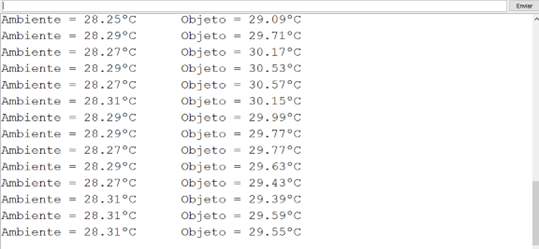
\includegraphics[width = \columnwidth]{Temperature_sensor_measurements.png}
                  \caption{Prueba de medición de temperatura de un objeto y del ambiente con el MLX90614}
                  \label{fig: temperature_measurements}
        \end{figure}
        \FloatBarrier 

        Como se observa en la figura \ref{fig: temperature_measurements} sobre el monitor serial, el sensor puede obtener la temperatura del 
        ambiente y el objeto, que en este caso será el bebé. Además es importante aclarar que el sensor viene calibrado de fabrica en un amplio rango de temperaturas de 
        -40 a 85 °C para la temperatura ambiente y -70 a 382.2 °C para la temperatura del objeto.\newline

        \textbf{Diagrama de conexión para el circuito}
        \begin{figure}[htp!]
            \centering
                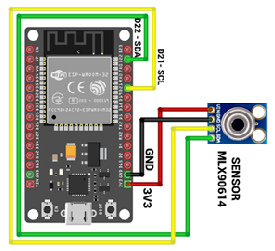
\includegraphics[width = 0.32 \textwidth]{wiring_diagram_mlx90614.png}
                \caption{Diagrama de conexiones entre el ESP32 y el MPU-9250}
            \end{figure}
            \FloatBarrier 
        \textbf{Código prueba}

        \lstset{style=mystyle}

        \lstinputlisting[language=C++, numbers=none]{temperature.cpp}
        
        \subsection{Duración de batería Li-Po}
        
        Las pruebas de duración fueron realizadas con el sensor de temperatura y el MPU conectados y obteniendo mediciones RAW 
        constantemente de ellos, con la batería que compramos se logró una autonomía de 15 horas sin necesidad de realizar alguna 
        optimización en el código para reducir consumo, esto nos da pauta bastante buena, ya que después de la optimización se 
        podran conseguir mejores tiempos.

        \begin{figure}[htp!]
            \centering
                 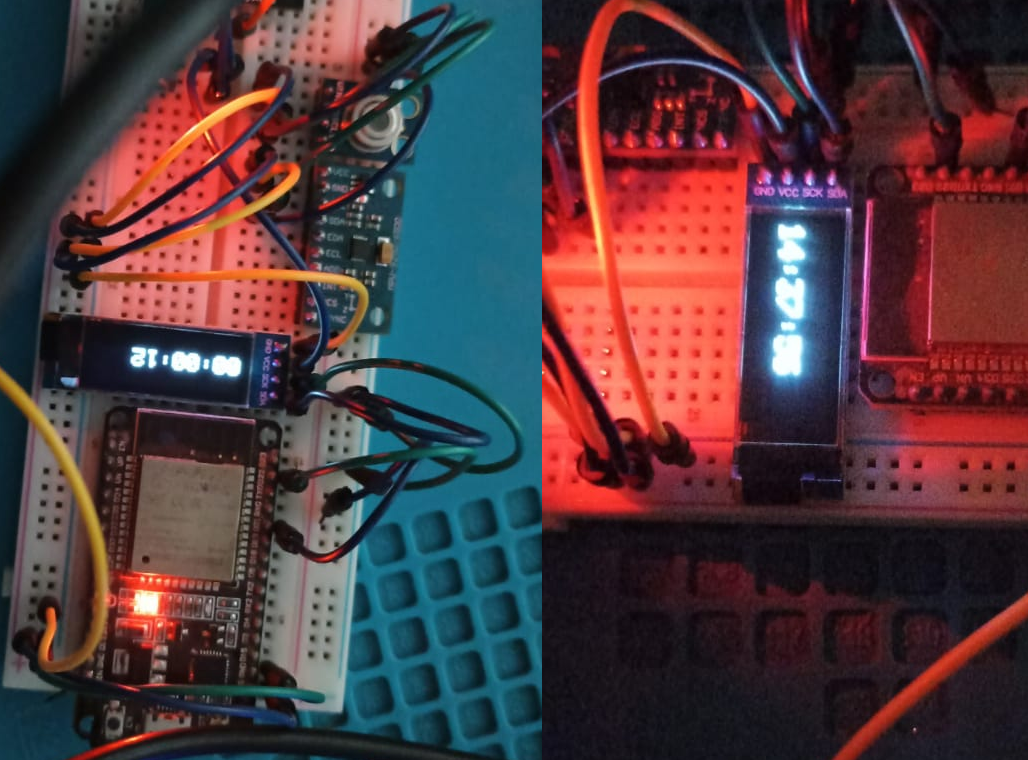
\includegraphics[width=\columnwidth]{battery_test.png}
                  \caption{Dos instantes de tiempo donde la batería aun tenía carga }
                  \label{fig: battery_test}
        \end{figure}
        \FloatBarrier

        En la figura \ref{fig: battery_test} se puede ver como la batería tuvo una muy buena duracion aun incluso sin tener optimizaciones
        el código.

